Los juegos de los que hablaremos son juegos para dos personas con información perfecta, sin movimientos al azar, y un resultado de ganar o perder. En estos juegos, los jugadores suelen alternar movimientos hasta alcanzar una posición terminal. Después de eso, un jugador es declarado ganador y el otro perdedor. La mayoría de los juegos de cartas no se ajustan a esta categoría, por ejemplo, porque no tenemos información sobre qué cartas tiene nuestro oponente.

\subsection{Ganar o perder}
Veamos es el siguiente juego, jugado por dos jugadores que se turnan para moverse. Al principio hay $n$ monedas. Cuando es el turno de un jugador, él puede quitar $m_1$, $m_2$, $m_3$, $\dots$  , $m_p$ monedas siendo $m_1 < m_2 < m_3 < \dots  < m_p$. El jugador que se lleva el último es declarado ganador (en otras palabras, el jugador que no puede hacer un movimiento es el perdedor). La pregunta es: ¿para qué $n$ ganará el primer jugador si ambos juegan de manera óptima ?.

Podemos ver que $n = m_1$, $m_2$, $m_3$, $\dots$, $m_p$ son posiciones ganadoras para el primer jugador, porque simplemente puede tomar todas las monedas. Para $n = 0$ no hay movimientos posibles (el juego está terminado), por lo que es la posición perdedora para el primer jugador, ya que no puede moverse de él. 

Supongamos que se puede quitar 1, 3 y 4 monedas podemos ver que n = 1, 3, 4 son posiciones ganadoras para el primer jugador, porque simplemente puede tomar todas las monedas. Para n = 0 no hay movimientos posibles (el juego está terminado), por lo que es la posición perdedora para el primer jugador, ya que no puede moverse de él. Si n = 2, el primer jugador tiene solo una opción, para eliminar 1 moneda. Si n = 5 o 6, un jugador puede moverse a 2 (eliminando 3 o 4 monedas), y está en una posición ganadora. Si n = 7, un jugador puede mover solo a 3, 4, 6, pero de todos ellos su oponente puede ganar.

Las posiciones tienen las siguientes propiedades:
\begin{itemize}
	\item Todas las posiciones terminales están perdiendo.
	\item Si un jugador puede moverse a una posición perdedora, entonces está en una posición ganadora.
	\item Si un jugador puede moverse solo a las posiciones ganadoras, entonces está en una posición perdedora.
\end{itemize}
Estas propiedades podrían usarse para crear un algoritmo WinLose-Algoritmo recursivo simple:

\begin{lstlisting}[language=C++]
logico esGanador(entero pos)
   //Posibles posiciones a las que puedo moverme desde la posicion pos;
   movs[]
   Por cada x que pertenece movs: 
      Si esGanador(x) == Falso: 
         retorno Verdadero
   retorno Falso
\end{lstlisting}

\begin{tabular}{|c|c|c|c|c|c|c|c|c|c|c|c|c|}
	\hline 
	n & 0 & 1 & 2 & 3 & 4 & 5 & 6 & 7 & 8 & 9 & 10 & 11 \\ 
	\hline 
	posición & L & W & L & W & W & W & W & L & W & L & W & W \\ 
	\hline 
	
\end{tabular} 

\vspace{0.5in}

Este juego podría jugarse también con una regla (generalmente llamada la regla de juego misere) de que el jugador que quita la última moneda es declarado perdedor. Solo necesita cambiar el comportamiento de las posiciones de terminal en el algoritmo WL. La tabla  cambiará a esto:


\begin{tabular}{|c|c|c|c|c|c|c|c|c|c|c|c|c|}
	\hline 
	n & 0 & 1 & 2 & 3 & 4 & 5 & 6 & 7 & 8 & 9 & 10 & 11 \\ 
	\hline 
	posición & W & L & W & L & W & W & W & W & L & W & L & W  \\ 
	\hline 
	
\end{tabular}
\vspace{0.5in}

Se puede ver que si una posición está ganando o perdiendo depende solo de las últimas $k$ posiciones, donde $k$ es el número máximo de monedas que podemos quitar. Si bien solo hay $2^{k}$ valores posibles para las secuencias de la longitud $k$, nuestra secuencia se volverá periódica.

\subsection{El juego del Nim}

El juego matemático más famoso es probablemente el Juego de Nim. Este es el juego que probablemente encontrarás más veces y hay muchas variaciones en él, así como juegos que se pueden resolver utilizando el conocimiento de cómo jugar el juego. Aunque estos problemas a menudo requieren una idea inteligente, generalmente son muy fáciles de codificar.

Históricamente, este juego fue popular en la antigüedad. Su origen probablemente esté en China, o al menos el juego Jianshizi es muy similar a él. En Europa las primeras referencias son del siglo XVI. El nombre se lo dio Charles Bouton, quien en 1901 publicó un análisis completo de este juego.

El juego clásico plantea que: Tenemos una pila con n piedras, y los jugadores pueden tomar de dicha pila, desde 1 hasta n piedras. El jugador que en su turno, no pueda retirar más piedras del bulto, se considera perdedor.

Está claro que siempre gana el jugador A, retirando todas las piedras, es decir, el jugador B alcanza un estado terminal que es un bulto con 0 piedras, por lo que podemos definir que la posición p = 0 es perdedora y que cualquier posición p > 0 es ganadora, porque podemos retirar todas las piedras y ganar.

Pero hagamos el juego más interesante, supongamos que cada jugador puede remover una o dos piedras solamente. La posición p = 0 sigue siendo una posición perdedora porque no podemos retirar ninguna piedra, fácilmente podemos ver que las posiciones p = 1 y p = 2 son ganadoras, simplemente retiramos todas las piedras. ¿Pero, qué sucedería si el bulto tiene 3 piedras?

De la posición p= 3 nos podemos mover a p = 2 retirando una piedra, y a p = 1 retirando dos piedras, ambas posiciones ganadoras para el próximo jugador a jugar, por lo tanto, p = 3 es perdedora.

Y si el bulto tuviera 4 piedras, ¿Cuántas piedras se podrían quitar?, ¿una o dos?. Si quitamos dos alcanzamos la posición p= 2 que es ganadora para el próximo jugador, y si quitamos una alcanzamos la posición p= 3 que es perdedora para el próximo jugador, así que la jugada óptima es quitar una sola piedra.

Entonces ya podemos definir dos conceptos importantes:

\textbf{Posición ganadora (G)}: Una posición es ganadora, si de esta podemos movernos al menos a una posición perdedora.

\textbf{Posición perdedora (P)}: Una posición es perdedora si de esta solo podemos movernos a posiciones ganadoras. Todos los estados terminales son posiciones perdedoras.

\begin{tabular}{|c|c|c|c|c|c|c|c|c|c|c|}
	\hline 
	n & 0 & 1 & 2 & 3 & 4 & 5 & 6 & 7 & 8 & 9  \\ 
	\hline 
	posición & P & G & G & P & G & G & P & G & G & P  \\ 
	\hline 
	
\end{tabular} 

En esta tabla se puede ver el patrón PGG, y llegar a la siguiente conclusión:

Definiendo P(n) como la posición del juego en el estado n.


P(n) = P (perdedora) si n es divisible por 3.


P(n) = G (ganadora) si n no es divisible por 3.

Variante del juego de Nim: Hay n pilas de monedas. Cuando es el turno de un jugador, él elige una pila y toma al menos una moneda de ella. Si alguien no puede moverse, pierde (por lo tanto, el que saca la última moneda es el ganador).

\begin{figure}
	\centering
	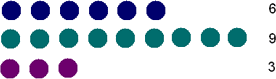
\includegraphics[scale=0.5]{img/juego_nim}
	\label{fig:juegonim}
	\caption{Juego del Nim}
\end{figure}

El estado del juego se describe sin ambigüedades mediante un conjunto múltiple de números enteros positivos. Un movimiento consiste en disminuir estrictamente un número entero elegido (si se convierte en cero, se elimina del conjunto).

La solución de Charles L. Bouton se ve así:

\textbf{Teorema:} El jugador actual tiene una estrategia ganadora si y solo si la suma xor de los tamaños 
de pila es distinta de cero. La suma xor de una sucesión $a$ es $a_1 \oplus a_2 \oplus \ldots \oplus a_n$, dónde $\oplus$ es el bit a bit exclusivo o.

\textbf{Prueba}. La clave de la prueba es la presencia de una estrategia simétrica para el oponente . Mostramos que una vez en una posición con la suma xor igual a cero, el jugador no podrá hacer que no sea cero a largo plazo, si hace la transición a una posición con una suma xor distinta de cero, el oponente siempre tendrá un movimiento que devuelve la suma xor a cero.

Probaremos el teorema por inducción matemática.

Para un Nim vacío (donde todas las pilas están vacías, es decir, el conjunto múltiple está vacío), la suma xor es cero y el teorema es verdadero.

Ahora supongamos que estamos en un estado no vacío. Usando el supuesto de inducción (y la aciclicidad del juego) asumimos que el teorema está probado para todos los estados alcanzables desde el actual.

Entonces la demostración se divide en dos partes: si para la posición actual el xor-sum $s = 0$, tenemos que demostrar que este estado está perdiendo, es decir, todos los estados alcanzables tienen xor-sum $t \neq 0$. Si $s \neq 0$, tenemos que probar que hay un movimiento que conduce a un estado con $t = 0$.

\begin{itemize}
	\item Dejar $s = 0$ y consideremos cualquier movimiento. Este movimiento reduce el tamaño de una pila $x$ a un tamaño $y$. Usando propiedades elementales de $\oplus$, tenemos
	
	$$t = s \oplus x \oplus y = 0 \oplus x \oplus y = x \oplus y$$
	
	Desde $y<x$ ,$y \oplus x$ no puede ser cero, entonces $t \neq 0$. Eso significa que cualquier estado alcanzable es ganador (por la suposición de inducción), por lo que estamos en una posición perdedora.
	
	\item Dejar $s \neq 0$ considere la representación binaria del número $s$. Dejar $d$ sea el índice de su bit principal (mayor valor) distino de cero. Nuestro movimiento será en una pila cuyo tamaño es el número de bit $d$ está establecido (debe existir, de lo contrario, el bit no se establecería en 
	$s$). Reduciremos su tamaño $x$ a $y = x \oplus s$. Todos los bits en posiciones mayores que $d$ en 
	$x$ y $y$ emparejar y morder $d$ está preparado $x$ pero no establecido $y$. Por lo tanto, $y<x$, que 
	es todo lo que necesitamos para que una mudanza sea legal. Ahora tenemos:
	
	$$t = s \oplus x \oplus y = s \oplus x \oplus (s \oplus x) = 0$$
	
	Esto significa que encontramos un estado perdedor alcanzable (por la suposición de inducción) y el estado actual es ganador.
\end{itemize}

\textbf{Corolario}. Cualquier estado de Nim puede ser reemplazado por un estado equivalente siempre que la suma xor no cambie. Además, al analizar un Nim con varias pilas, podemos reemplazarlo con una sola pila de tamaño $s$.

